\documentclass[11pt]{report}
\usepackage[margin=2.3cm]{geometry}
\usepackage[fleqn]{amsmath}
\usepackage{nccmath}
\usepackage{alltt}
\usepackage{sectsty}
\usepackage{titlesec}
\newcommand{\ts}{\textsuperscript}
\usepackage{graphicx}
\graphicspath{ {../images/} }
\usepackage{subfig}
\usepackage[hidelinks]{hyperref}
\newcommand{\linespace}{\vspace{0.3cm}\noindent}

\titlespacing*{\section}{0pt}{0.8\baselineskip}{0.2\baselineskip}

\begin{document}

\begin{titlepage}
    \begin{center}
        \vspace*{1cm}
        
        \textbf{CO3093 COURSEWORK 2 - Report}
        
        \vspace{0.5cm}
		Big Data \& Predictive Analytics - Classification \& Clustering
        
        \vspace{1.5cm}
        
        \textbf{Ihtasham Chaudhry}
        
        \vfill
        
        \vspace{0.8cm}
                
        Department of Informatics\\
        University of Leicester\\
        28\ts{th} March 2018
        
    \end{center}
\end{titlepage}

\newpage

\section{Exploring the data}

\linespace
In this section we will explore the data-set \texttt{Diabetes 130-US hospitals for years 1999-2008}. 

\subsection{Exploring the data as a whole}

To visualise and explore the data-set it's important to extract key-information as some of the columns in the data-set are not key in analysing the data.

\linespace
Firstly, we must remove any rows/columns that have missing values and that we may not be able to use in order to conduct any further experiments or analysis on. There seem to be many rows with \texttt{?} values, i.e. unknown values and mostly on the columns \texttt{weight} and \texttt{payer\_code}. So we can remove these as they will not be relevant in either clustering or analysing the data-set.

\linespace
From the numerical data we can make the following analyses:

\begin{itemize}
	\item The mean time spent in hospital by a patient who has been admitted is approximately 4 days. 
\end{itemize}

\linespace
At a basic level we can visualise the distribution of diabetic patients by race and gender, the results of this can be seen below.

\begin{figure}[ht]
	\begin{minipage}[b]{.5\textwidth}
	\centering
	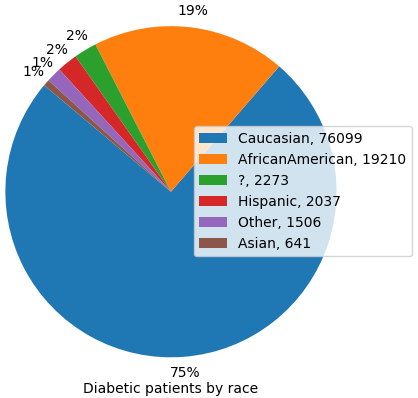
\includegraphics[width=1\textwidth]{race_pie.png}
	\caption{Proportion of diabetics by race}
	\end{minipage}
	\hfill
	\begin{minipage}[b]{.5\textwidth}
	\centering
	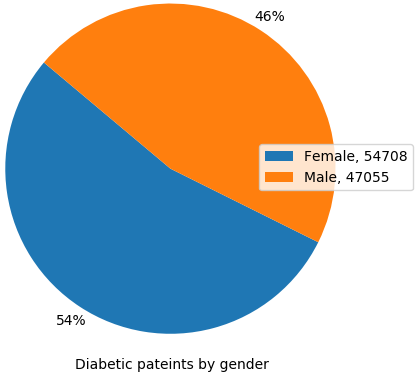
\includegraphics[width=1\textwidth]{gender_pie.png}
\caption{Proportion of diabetics by gender}
\end{minipage}
\end{figure}

\linespace
From this we can see that majority of diabetic patients admitted to US hospitals from 1999 to 2008 are mostly Caucasian (75\%) by analysing the gender split, it's almost equal split however a higher percentage of females (54\%) than males (46\%).
  
\end{document}